\documentclass[../main.tex]{subfiles}
\graphicspath{{\subfix{../images/}}}
\begin{document}

\subsection{Investigating of AlexNet}

The CNN Model have been a model in use for a long time for training models to identify images. One such instance to classify images in the ImageNet database. The ImageNet database has 1000 classes and contains 1,281,167 training images, 50,000 validation images and 100,000 test images. Using this database, ImageNet hosted the competition, ImageNet Large Scale Visual Recognition Challenge (ILSVRC), that asked its contestants to submit a model that can classify the object within the images of this database.  \cite{ILSVRC15}

One of the contestants was AlexNet in 2012. The AlexNet CNN model achieved an error rate of 15.3\% on the ImageNet database with the second best achieving 26.2\%. AlexNet has several properties used in its model.  \cite{alexnet}

\subsubsection{ReLU}
As oppose to the tanh function or the sigmoid function which were common at the time, AlexNet used the ReLU function \begin{equation*}
f(x) = \left\{
        \begin{array}{ll}
            0 & \quad x \leq 0 \\
            x & \quad x \geq 0
        \end{array}
    \right.
\end{equation*}

From their findings, using the ReLU function reduced the error in fewer iterations than the other functions. It was tested that the ReLU function achieved a 25\% error rate on the CIFAR-10 dataset in fewer epochs than the other 2 alternatives. This is beneficial as faster learning prevents overfitting of the model. \cite{alexnet}

\subsubsection{Overlapping Pools}
Usually during the pooling process, adjacent pools do not overlap however, in AlexNet, overlapping pools were used. This means the outputted array will be larger as extra pixels between adjacent pools will be added. The use of the overlapping pools prevented overfitting from the AlexNet model slightly so adding this into the network could be beneficial.  \cite{alexnet}

\subsubsection{Data Augmentation}
AlexNet augmented its data by converting it to size 256x256 images then cropping the center 224x224 pixels to be used in the model. This means that a the edges of the images were discarded which makes sense to do as the focus is going to be in the center and removing part of the border also removes unnecessary noise from the image.  \cite{alexnet}

\subsubsection{Dropout Layers}
A regulation technique used by the AlexNet model was the dropout technique. What happens at this layer is that every node is given a 50\% chance of outputting 0 instead of its usual output. This means that the node will not participate in back propagation. This essentially samples a range of network architectures and the model must be trained to use all nodes to inform its output. This prevents overfitting as the model will teach the model to find alternative patterns in the data. This is at the expense of the model needing to complete double the number of iterations to converge. AlexNet used dropout in the first 2 convolutional layers. \cite{alexnet}

\subsubsection{Architecture}
\begin{figure}[h!]
  \centering
  \begin{subfigure}[b]{0.8\linewidth}
    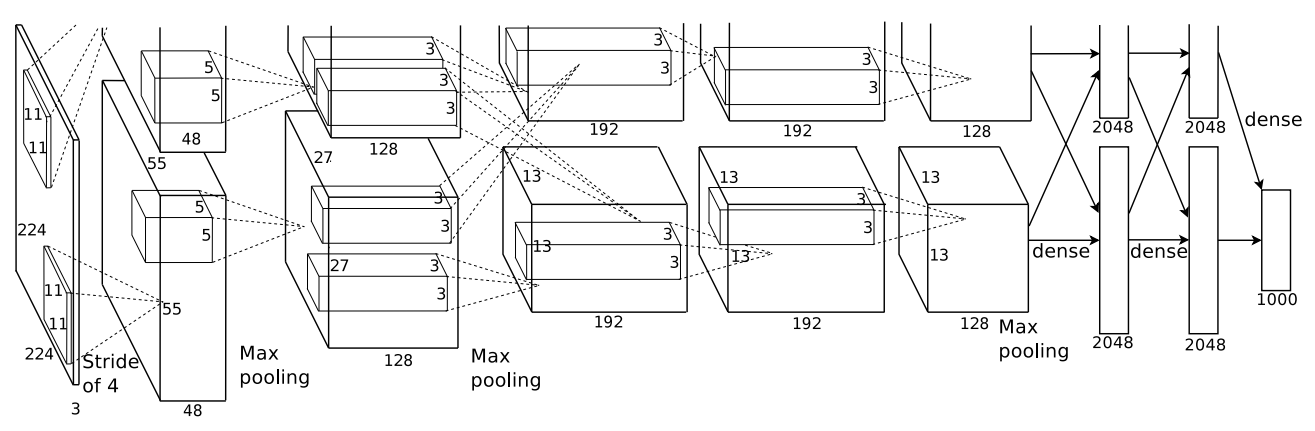
\includegraphics[width=\linewidth]{alexnet.png}
  \end{subfigure}
  \caption{AlexNet model architecture}
  \label{fig:alexnet}
\end{figure}

In the AlexNet paper, an image of the CNN architecture was provided where its inner workings can be examined. It can be seen that the kernel size at the convolutional layer varied with the largest being 11 for the first layer then reducing to 5 then 3 in the later layers. We also see the use of strides which is a variable that determines how much to move the kernel each time. It can also been see that the number of layers extracted is quite large with the most layers at one point being 192 layers.

\end{document}